\documentclass[border=10pt]{standalone}
\usepackage[svgnames]{xcolor}
\usepackage{amsmath}
\usepackage{pgfplots}
\pgfplotsset{compat=newest}
\usepackage[sfdefault]{FiraSans}
\usepackage{FiraMono}
\renewcommand*\familydefault{\sfdefault}
\begin{document}
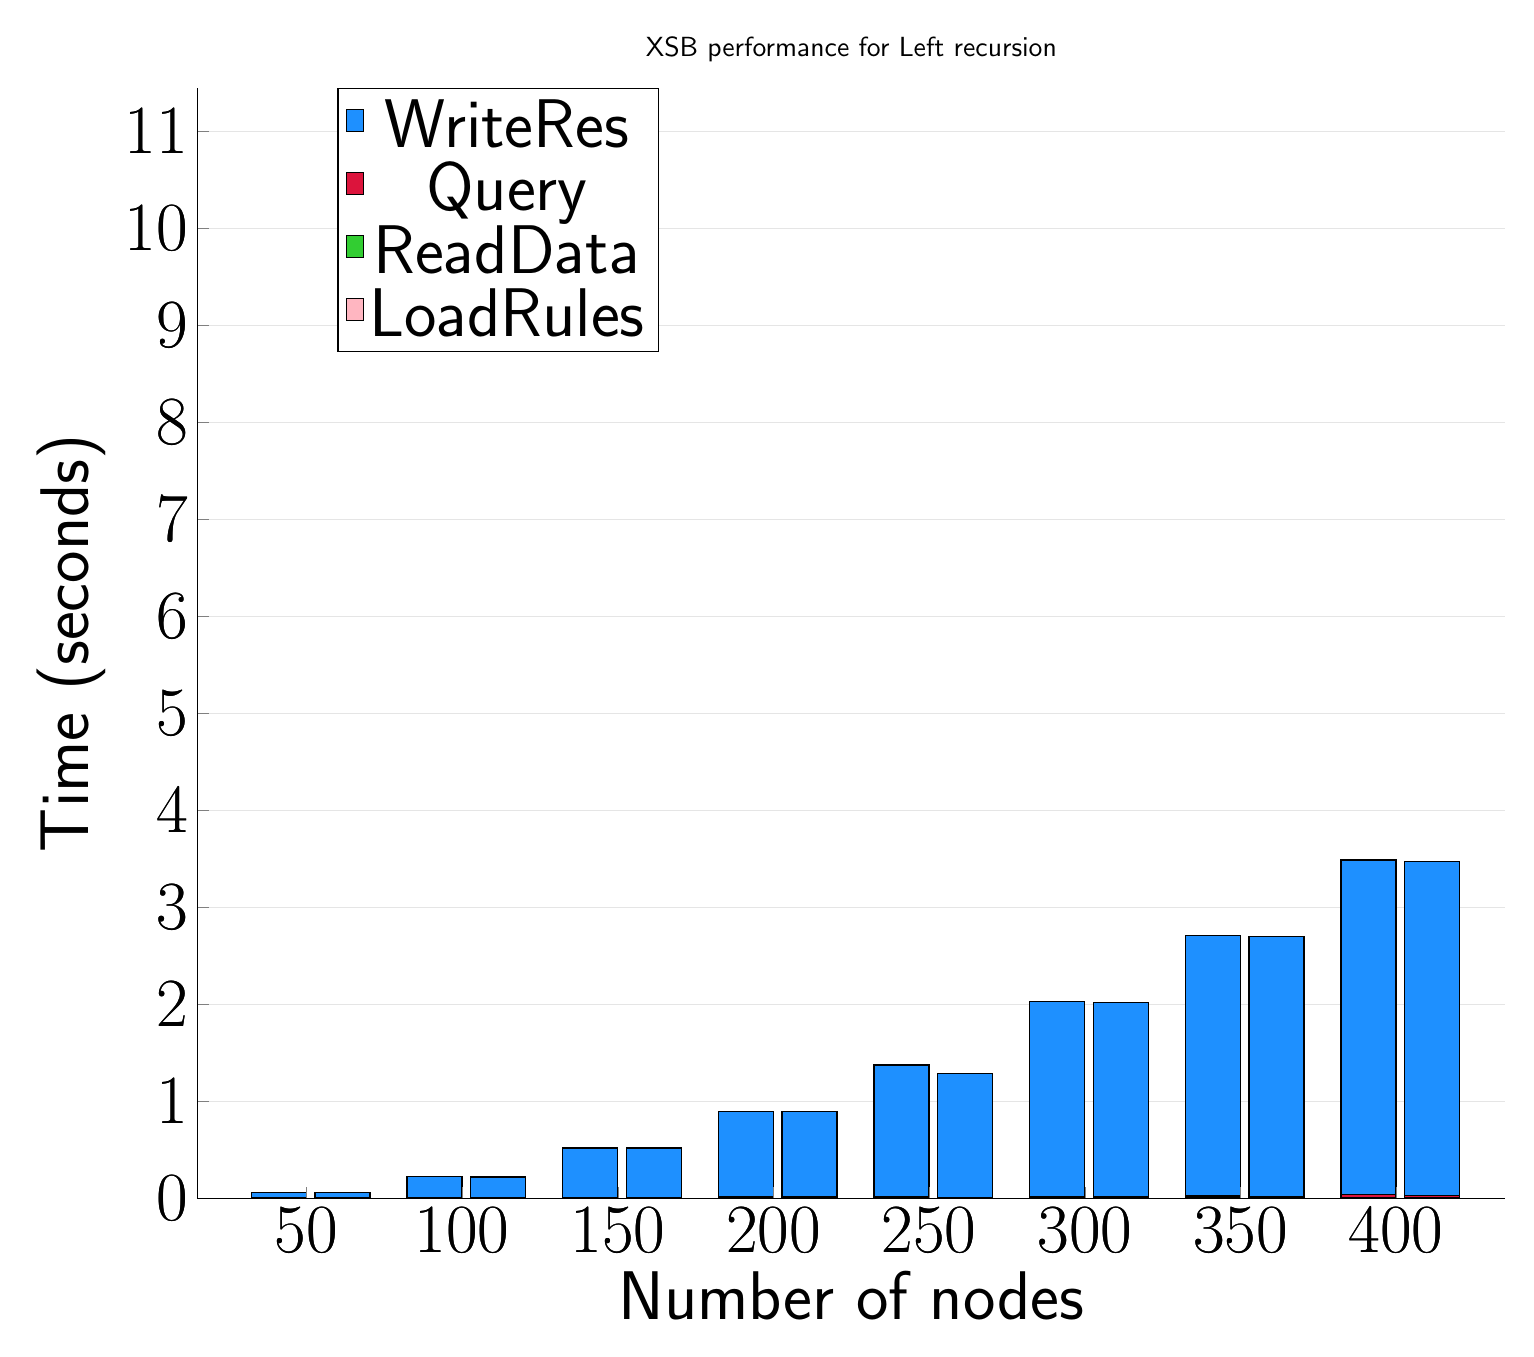
\begin{tikzpicture}
\begin{axis}[
   ybar stacked,
   title={XSB performance for Left recursion},
   bar shift=-10pt,
   width=1.5\textwidth,
   bar width=0.7cm,
   ymajorgrids, tick align=inside,
   major grid style={draw=gray!20},
   xtick=data,
   ymin=0, ymax=11.449559211730957,
   axis x line*=bottom,
   axis y line*=left,
   enlarge x limits=0.1,
   legend style={
       at={(0.23, 1)},
       anchor=north,
       legend columns=1,
       font=\Huge,
   },
   ylabel={Time (seconds)},
   xlabel={Number of nodes},
   label style={font=\Huge},
   tick label style={font=\Huge},
]
\addlegendimage{fill=DodgerBlue, draw=black, line width=0.2pt}
\addlegendentry{WriteRes}
\addlegendimage{fill=Crimson, draw=black, line width=0.2pt}
\addlegendentry{Query}
\addlegendimage{fill=LimeGreen, draw=black, line width=0.2pt}
\addlegendentry{ReadData}
\addlegendimage{fill=LightPink, draw=black, line width=0.2pt}
\addlegendentry{LoadRules}
\addplot +[fill=LightPink, draw=black, line width=0.5pt] coordinates {
    (50, 0.004476706186930337)
    (100, 0.00485110282897949)
    (150, 0.005252679189046224)
    (200, 0.005396922429402671)
    (250, 0.0038583278656005864)
    (300, 0.00452907880147298)
    (350, 0.004204591115315757)
    (400, 0.004375060399373374)
};
\addplot +[fill=LimeGreen, draw=black, line width=0.5pt] coordinates {
    (50, 0.0019339720408121733)
    (100, 0.0025363763173421234)
    (150, 0.0037636756896972635)
    (200, 0.004712104797363284)
    (250, 0.00398103396097819)
    (300, 0.00522828102111816)
    (350, 0.006119330724080403)
    (400, 0.00698590278625488)
};
\addplot +[fill=Crimson, draw=black, line width=0.5pt] coordinates {
    (50, 0.0003392696380615234)
    (100, 0.0014225641886393234)
    (150, 0.0035146077473958335)
    (200, 0.0065582593282063764)
    (250, 0.007223924001057942)
    (300, 0.0127530892690023)
    (350, 0.01795037587483723)
    (400, 0.0285184383392334)
};
\addplot +[fill=DodgerBlue, draw=black, line width=0.5pt] coordinates {
    (50, 0.05523800849914551)
    (100, 0.21747469902038566)
    (150, 0.5100807348887125)
    (200, 0.8826254208882652)
    (250, 1.3621509869893387)
    (300, 2.007504701614381)
    (350, 2.680874903996786)
    (400, 3.449559211730957)
};
\end{axis}
\begin{axis}[
   ybar stacked,
   bar shift=13pt,
   width=1.5\textwidth,
   bar width=0.7cm,
   ymajorgrids, tick align=inside,
   major grid style={draw=none},
   xtick=data,
   ymin=0, ymax=11.449559211730957,
   axis x line*=none,
   axis y line*=none,
   enlarge x limits=0.1,
   label style={font=\Huge},
   tick label style={font=\Huge},
]
\addplot +[fill=LightPink, draw=black, line width=0.5pt] coordinates {
    (50, 0.0040120000000000025)
    (100, 0.00481366666666667)
    (150, 0.004752333333333333)
    (200, 0.005040333333333337)
    (250, 0.003108666666666667)
    (300, 0.00389433333333334)
    (350, 0.0037883333333333332)
    (400, 0.0033330000000000005)
};
\addplot +[fill=LimeGreen, draw=black, line width=0.5pt] coordinates {
    (50, 0.0016073333333333235)
    (100, 0.0023743333333333333)
    (150, 0.0036070000000000065)
    (200, 0.004365000000000001)
    (250, 0.003822333333333334)
    (300, 0.0050683333333333335)
    (350, 0.005576666666666667)
    (400, 0.004511999999999999)
};
\addplot +[fill=Crimson, draw=black, line width=0.5pt] coordinates {
    (50, 0.0003023333333333327)
    (100, 0.001279333333333327)
    (150, 0.0035156666666666635)
    (200, 0.006404333333333337)
    (250, 0.007226999999999997)
    (300, 0.012758)
    (350, 0.014266666666666669)
    (400, 0.024838666666666665)
};
\addplot +[fill=DodgerBlue, draw=black, line width=0.5pt] coordinates {
    (50, 0.053944)
    (100, 0.21452433333333334)
    (150, 0.5101436666666667)
    (200, 0.8802796666666667)
    (250, 1.2762033333333334)
    (300, 2.0020466666666668)
    (350, 2.6777953333333335)
    (400, 3.440412333333333)
};
\end{axis}
\end{tikzpicture}

\end{document}
